% Created 2015-01-09 Fri 23:54
\documentclass[11pt]{article}
\usepackage[utf8]{inputenc}
\usepackage[T1]{fontenc}
\usepackage{fixltx2e}
\usepackage{graphicx}
\usepackage{longtable}
\usepackage{float}
\usepackage{wrapfig}
\usepackage{soul}
\usepackage{textcomp}
\usepackage{marvosym}
\usepackage{wasysym}
\usepackage{latexsym}
\usepackage{amssymb}
\usepackage{hyperref}
\tolerance=1000
\providecommand{\alert}[1]{\textbf{#1}}

\title{Lecture 11 Notes}
\author{Nooreen Dabbish}
\date{\today}
\hypersetup{
  pdfkeywords={},
  pdfsubject={},
  pdfcreator={Emacs Org-mode version 7.9.3f}}

\begin{document}

\maketitle



\section{Cheatsheet codesamples}
\label{sec-1}
\subsection{From orgmode tutorials\ldots{}}
\label{sec-1-1}


*Playing with Org-mode-R:

\begin{verbatim}
plot(matrix(rnorm(100), ncol=2), type="l")
\end{verbatim}


\begin{verbatim}
library(ascii)
options(asciiType="org")
ascii(summary(table(1:4, 1:4)))
\end{verbatim}


\begin{verbatim}
library(ascii)
a <- runif(100)
c <- "Quantiles of 100 random numbers"
b <- ascii(quantile(a),header=T,include.colnames=T,caption=c)
print(b,type="org")
rm(a,b,c)
\end{verbatim}


\begin{verbatim}
library(ggplot2)
# create factors with value labels 
mtcars$gear <- factor(mtcars$gear,levels=c(3,4,5),
        labels=c("3gears","4gears","5gears")) 
mtcars$am <- factor(mtcars$am,levels=c(0,1),
        labels=c("Automatic","Manual")) 
mtcars$cyl <- factor(mtcars$cyl,levels=c(4,6,8),
   labels=c("4cyl","6cyl","8cyl")) 

# Kernel density plots for mpg
# grouped by number of gears (indicated by color)
qplot(mpg, data=mtcars, geom="density", fill=gear, alpha=I(.5), 
   main="Distribution of Gas Milage", xlab="Miles Per Gallon", 
   ylab="Density")

if(FALSE){# Scatterplot of mpg vs. hp for each combination of gears and cylinders
# in each facet, transmittion type is represented by shape and color
qplot(hp, mpg, data=mtcars, shape=am, color=am, 
   facets=gear~cyl, size=I(3),
   xlab="Horsepower", ylab="Miles per Gallon") 

# Separate regressions of mpg on weight for each number of cylinders
qplot(wt, mpg, data=mtcars, geom=c("point", "smooth"), 
   method="lm", formula=y~x, color=cyl, 
   main="Regression of MPG on Weight", 
   xlab="Weight", ylab="Miles per Gallon")

# Boxplots of mpg by number of gears 
# observations (points) are overlayed and jittered
qplot(gear, mpg, data=mtcars, geom=c("boxplot", "jitter"), 
   fill=gear, main="Mileage by Gear Number",
   xlab="", ylab="Miles per Gallon")}
\end{verbatim}


\begin{verbatim}
library(xtable)
x <- rnorm(100)
y <- x + rnorm(100)
xtable(summary(lm(y ~ x)))
\end{verbatim}
\subsection{From Random}
\label{sec-1-2}

(-1.96< Z < 1.96)


\begin{center}
\begin{tabular}{rrr}
 Y  &  X  &  Z  \\
\hline
 1  &  2  &  3  \\
\end{tabular}
\end{center}





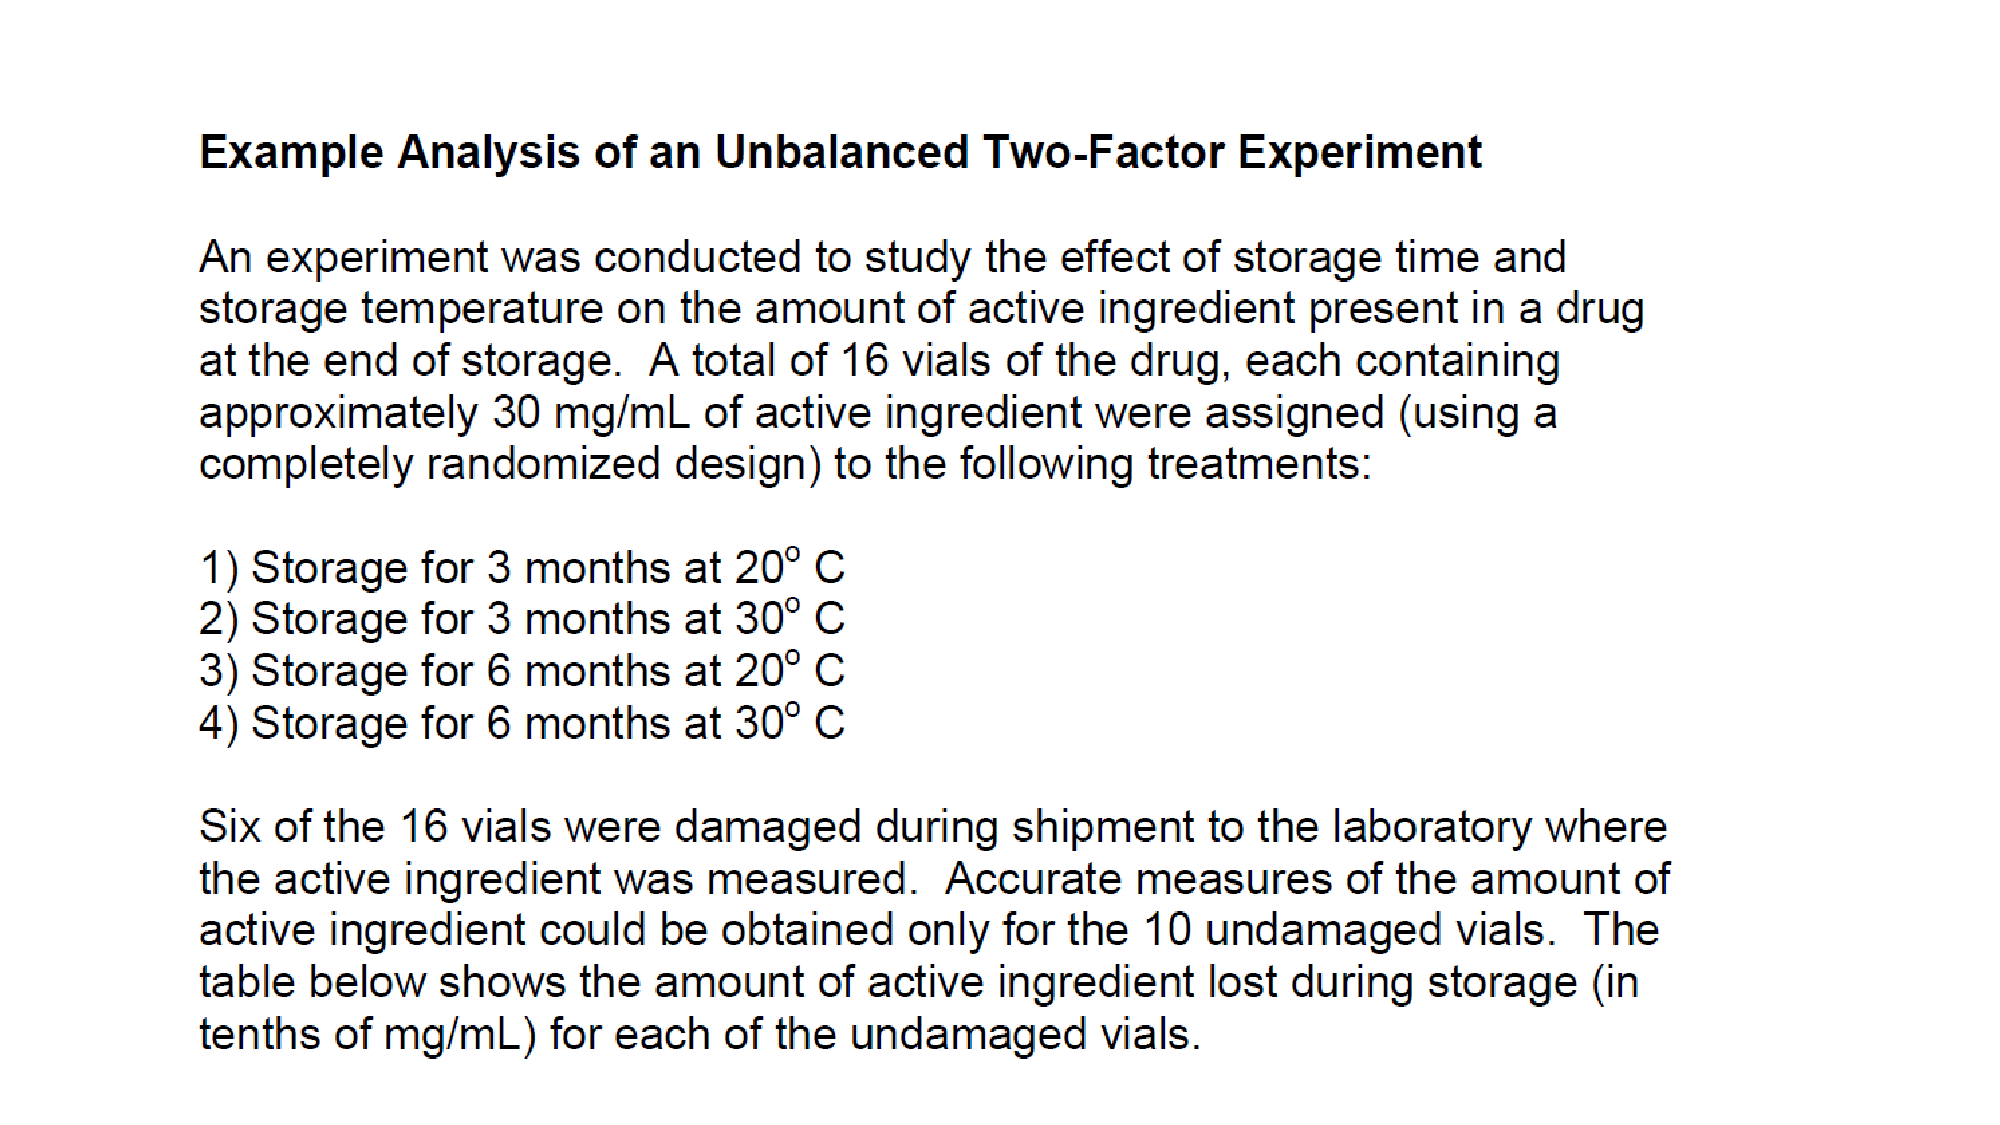
\includegraphics[width=.9\linewidth]{example.pdf}
\subsection{From a HW}
\label{sec-1-3}
\subsubsection{Plot Histograms of Time and Log(Time-3100)}
\label{sec-1-3-1}



\begin{figure}[p]
\centering
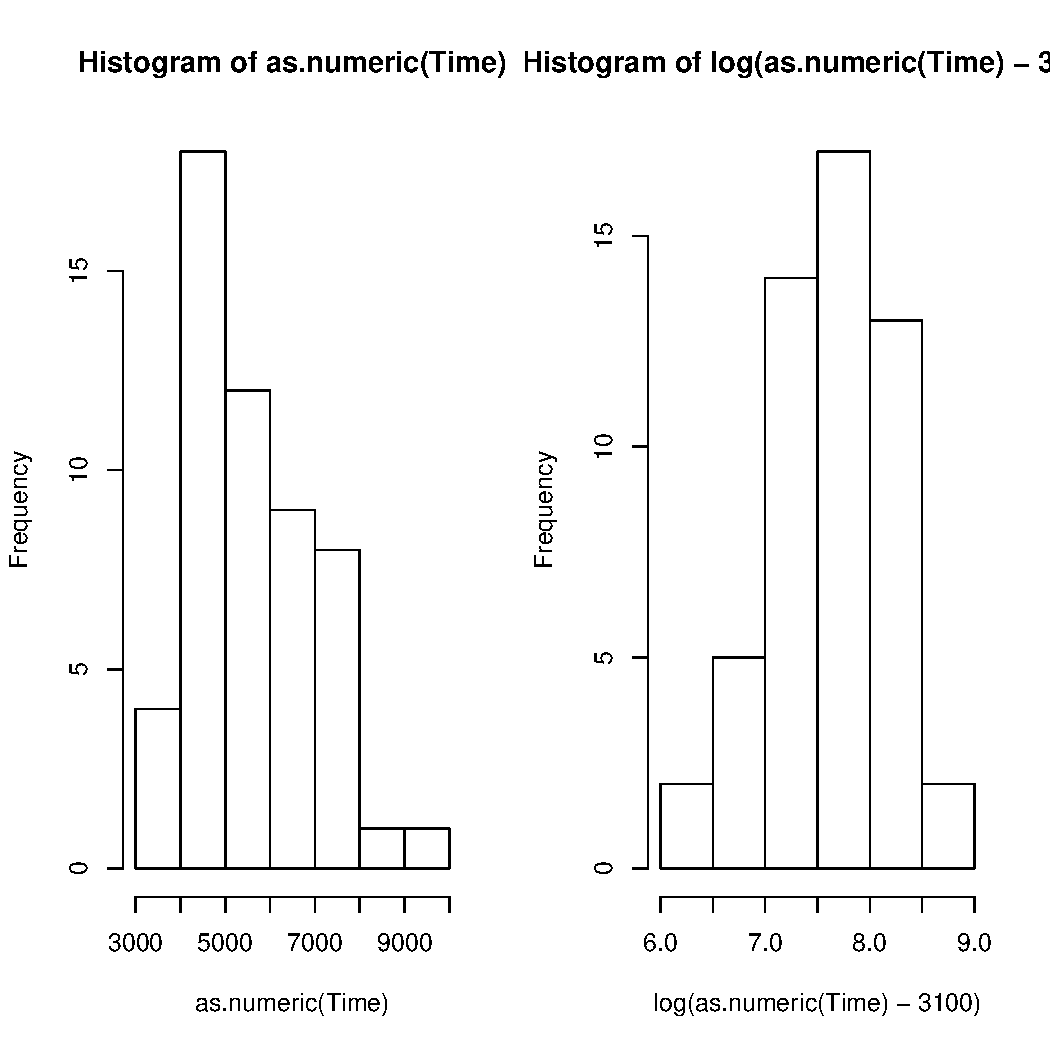
\includegraphics[width=0.8\textwidth,]{prob2a.pdf}
\caption{\label{fig:histograms}Histograms of Yacht Data}
\end{figure}
\subsubsection{Plot a scatterplot log(Time - 3100) vs. Year}
\label{sec-1-3-2}



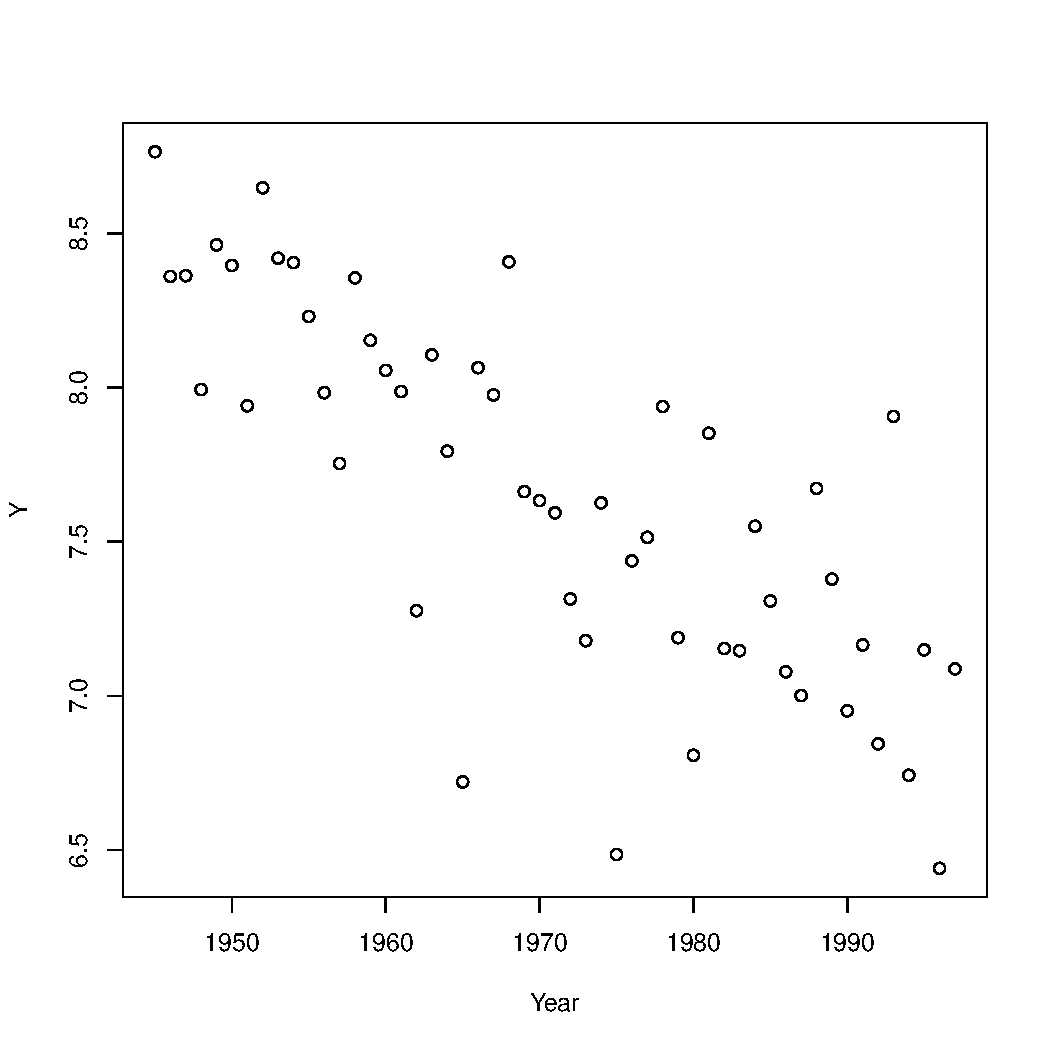
\includegraphics[width=.9\linewidth]{prob2b.pdf}
\begin{itemize}

\item Write out a linear model to study the relationship between log(Time - 3100) and Year.\\
\label{sec-1-3-2-1}%
Interpret your two parameters in the model.

\begin{align*}
\mathrm{Let} Y_i &= log(\mathrm{Time}_i -3100)\\
\mathrm{Model:} Y_i = \beta_0 + \beta_1 X_i + \epsilon_i\\
\hat{\beta}_1 &= \frac{S_{xy}}{S_{xx}} \\
              &=\frac{ \sum (X_i - \bar{X})(Y_i - \bar{Y})}{\sum (X_i - \bar{X})^2}\\
              &= -0.03\\
\hat{\beta}_{0} &= \bar(Y) - \hat{\beta}_{1}\bar{X}\\
              &= 65.64
\end{align*}

\textbf{Interpretation:} $\beta$$_0$ tells us the value of Y when/if X equals 0.
So in year 0, we would expect $\log(\mathrm{Time} - 3100)$ to be
approximately 66. Solving for Time gives \texttt{3.2226970275426e+28}.

$\beta$$_1$ tells us the magnitude of increase in $\log(\mathrm{Time} -
3100)$ for a 1 year increase in time. Since $\beta$$_0$ is negative, it
is actually a decrease. Solving for Time gives \texttt{3100.97}


\end{itemize} % ends low level
\section{Concepts to review}
\label{sec-2}
\subsection{Matrix}
\label{sec-2-1}

\begin{itemize}
\item $\Box$ Positive definite, relationship to full rank if any?
\item $\Box$ projection matrices
\item $\Box$ Orthogonal matrix
\end{itemize}
\subsection{Concepts}
\label{sec-2-2}
\subsubsection{Multiple Linear Regression}
\label{sec-2-2-1}

\begin{itemize}
\item $\boxtimes$ Show that $\hat{\beta}$ is unbiased.
\item $\boxtimes$ Why is $Var(\hat{\beta}) = \sigma^2 (\mathbf{X}^T\mathbf{X})^{-1}$
    $Var(\mathbf{A}\mathbf{X}) = \mathbf{A} Var(\mathbf{X})
  \mathbf{A}^{T}$
    Why is the variance of \textbf{X$\beta$} 0?
\item $\boxtimes$ Gauss Markov Theorem
    BLUE
\end{itemize}
\subsubsection{SLR/MLR connection}
\label{sec-2-2-2}

\begin{itemize}
\item $\Box$ Reread
\item $\Box$ Do HW problem
\end{itemize}

\end{document}
